
\subsection{Combining Power control and Load balancing}

\subsubsection{Online max-min (OMM)}
% OUT OF PLACE
\begin{figure*}
\centering
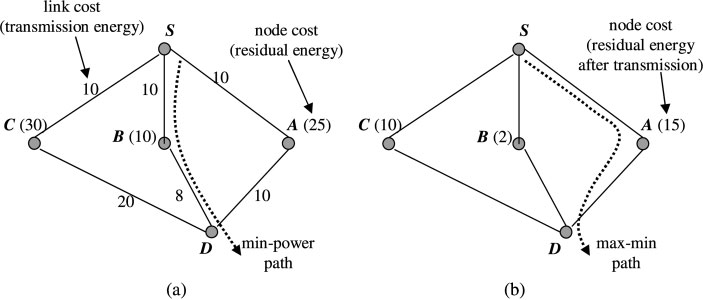
\includegraphics[width=0.7\textwidth]{images/omm}
\caption{Paths in OMM\cite{alotaibi2012survey}}
\label{ommex}
\end{figure*}
\label{omm}
OMM \cite{li2001online} maximises the network lifetime using two metrics:
\begin{enumerate}
  \item \textbf{min-power} - Minimising the overall power
  \item \textbf{max-min} - Maximising the minimum residual power after a transmission
\end{enumerate}

First OMM calculates the \textit{min-power} path using Dijkstra’s algorithm. Let
the power required by that be $P_{min}$.
It then determines the \textit{max-min} paths by looking at all paths whose
power do not deviate much from the min-power path; that is, those paths which consume less
power than $zP_{\min}$ for some $z \ge 1$. It calculates the minimum residual power of all nodes
after the transmission would have taken place, and chooses the path where
that value is largest.

For example, in Figure~\ref{ommex}, the min-power path from
$S$ to $D$ is $S \to B \to D$ with a value of 18 ($S \to A \to D$ has 20,
$S \to C \to D$ has 30).
It's minimum residual energy will be $2$, as node $B$ needs
$8$ out of the $10$ power units it has.

Looking at the alternate paths, $S \to C \to D$ will have a
minimum residual energy of $30-20=10$ in node $C$, and $S \to A \to D$ will
have a minimum residual energy of $25-10$ in node $A$.
Thus, the max-min path is $S \to A \to D$.

Choosing a good value for $z$ in $zP_{\min}$ is important: For $z=1$, only
the min-power path is considered; for $z \to \inf$, all paths can be
considered. The algorithm starts with a \textit{random} value for $z$, and
then measures the residual energy (\textit{lifetime}) of of the most overloaded node during some
fixed time period.

 Afterwards, the value of $z$ is increased by a small constant
 and the lifetime is measured again. If the lifetime increases, the value of $z$
is increased; otherwise, it is decreased.

Because the lifetime is measured
in two distinct time periods, it is assumed that load distribution is roughly
similar, otherwise the results might not be really useful.
%OOP: SPAN-FIGURE
\begin{figure*}
\centering
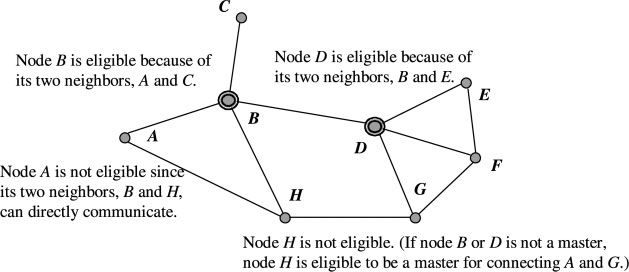
\includegraphics[width=0.8\textwidth]{images/span-master-example}
\caption{Master eligibility rule in the SPAN protocol\cite{alotaibi2012survey}}
\label{spanmaster}
\end{figure*}
\subsubsection{Conditional max-min battery capacity routing (CMMBCR)}
Like LEAR, CMMBCR\cite{toh2001maximum} uses a threshold level to optimise
the energy effiency of its routing.
Unlike LEAR, the threshold is fixed, though.

If all nodes in some paths have higher residual energy than the threshold,
the min-power path is chosen.

If all routes have nodes with a residual energy lower than the threshold, the
max-min route will be selected.

\subsubsection{Dynamic Source Routing Power-Aware (DSRPA)}
\label{dsrpa}
Dynamic Source Routing Power-Aware (DSRPA)\cite{djenouri2006new} defines a
power-aware variant of dynamic source routing.

It uses a trade off between the `freshness' of batteries, that is, how much
energy is still left in them; and the power consumption of the route, by
defining a metric involving those two factors, and using that to measure the
cost of a route.

Power consumption is reduced by recording the transmission power in route
request messages and then using that value and the reception power to calculate
the required power for transmitting a packet to the sender at the receiver side.

A node can share its power state by broadcasting in its neighbourhood a special
$E_{state}$ packet that contains the current power value. This packet is send
each time a certain percentage of power has been consumed. For example, if the
rate is set to $25\%$, a packet will be sent after 25, 50, and 75 per cent of
power consumed.

A route $c=I_{0}, \ldots, I_{n-1}$ is considered optimal if its value $Opt_{c}$,
as defined in  (\ref{eq:dsrpa:opt-c}) is the minimum for all routes. Routes can
be totally ordered using that value, giving us the ability to disperse data
among several routes (see below).
\begin{align}
Opt_{c} &:= \sum_{i=0}^{n-2} \frac{\alpha}{\underbrace{1-eng(I_{i})}_{\text{residual energy rate}}} + \frac{1-\alpha}{\underbrace{1-\frac{Pow(I_{i}, I_{i+1})}{MaxPow(I_{i})}}_{= 1 - \text{rate of total power}}}
\label{eq:dsrpa:opt-c}
\end{align} 
The factors in  (\ref{eq:dsrpa:opt-c}) have the following meanings:
\begin{itemize}
    \item $\alpha$ is a weight
    \item $eng(I_{i}) \in [0,1]$ is the rate of energy consumed by $I_{i}$,
    \item $Pow(I_{i}, I_{i+1})$ is the power required for the link from $I_{i}$ to $I_{i+1}$, and
    \item $MaxPow(I_{i})$ is the maximum power of the node $I_{i}$, that is, the power that allows
          it to cover its power range.
\end{itemize}


The more $\alpha$ increases, the more nodes with fresh batteries are preferred
(and the more $\alpha$ decreases, the more min-power routes are preferred).

$\alpha$ can be defined as a function of time (\ref{eq:dsrpa:alpha}),
for some $EngDiff \in [0,1]$ accounting for the difference between the maximum and minimum rate
of energy consumed in the network and some $\alpha_{0}$ as the initial value.
\begin{align}
    \alpha &:= \sqrt{(1-\alpha_{0})^{2} \cdot EngDiff + \alpha_{0}}
    \label{eq:dsrpa:alpha}
\end{align}

This counters the increasing difference $EngDiff$ because if that
difference increases, $\alpha$ increases, and thus fresher nodes are preferred,
and therefore, the value of $EngDiff$ decreases.

DSRPA disperses data over multiple routes.  While normal DSR only uses one
`optimal' route, DSRPA can discover and use multiple nodes if the route request
packet contains a \texttt{ALLROUTES} flag.

It will then use non-optimal routes to distribute the load of the network like
this:

If $\#packets$ is the number of packets to be sent and
$\#paths$ is the number of paths from the source to the
destination, and the routes are ordered according to their optimality,
with 0 being the best, then the number of packets to be sent on the route $i$
is given by (\ref{eq:dsrpa:packets}).
\begin{align}
     \#packets_{i} &:= \left\lceil \frac{2^{\# paths - i - 1} \cdot \# packets}{2^{\#paths} - 1} \right\rceil
     \label{eq:dsrpa:packets}
\end{align}

This ensures that most packets are delivered on the optimal route $i=0$, and
the package count in a less optimal route is less than the count in a more
optimal route. The number of packets send on a route $i$ is approximately
twice as much as the number of packets send on the route $i+1$.

The data dispersal requires more energy than would be needed without it. It
does however minimise the difference in energy states. The decision of whether
to use data dispersal or not must be made on a per-network basis: Networks
enjoying high connectivity will consume more power with data dispersal than
networks with low connectivity, because there will be a lot more broadcasting.
